% Slide 223
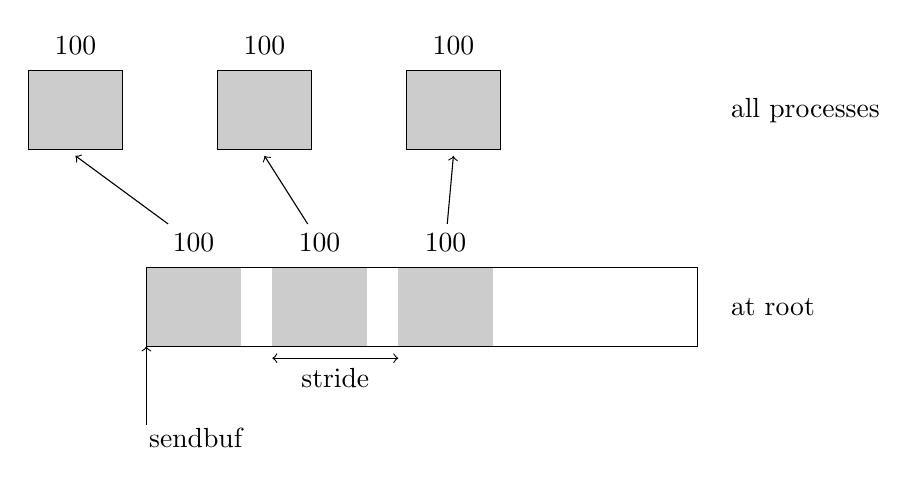
\begin{tikzpicture}

\foreach \x in {0, 1.6, 3.2} {
	\fill[gray!40!white] (\x, 0) rectangle (\x + 1.2, 1);
	\node[anchor = south] (N) at ({(2 * \x + 1.2)/ 2}, 1.08) {100};

	\pgfmathsetmacro{\xtop}{1.5 * (\x - 1)}
	\pgfmathsetmacro{\xmid}{(2 * \xtop + 1.2)/ 2}
	\draw[fill = gray!40!white] ({\xtop}, 2.5) rectangle ({\xtop + 1.2}, 3.5);
	\node[anchor = south] at (\xmid, 3.58) {100};

	\draw[->] (N) -- (\xmid, 2.42);
}

\draw (0,0) rectangle (7, 1);

\node[anchor = west] at (7.3, 0.5) {at root};
\node[anchor = west] at (7.3, 3) {all processes};

\node[anchor = north west, outer sep = 0pt, inner sep = 1pt] (S) at (0, -1) {sendbuf};
\draw[->] (S.north west) -- (0,0);

\draw[<->] (1.6, -0.15) -- node[midway, below] {stride} (3.2, -0.15);

\end{tikzpicture}
